\section{Business understanding} \label{seq:business}

 In this phase the objective is to determine and understand the context and the scope of the project. So it has a lot in common with the initial steps of any significant project undertaking.

\begin{figure}[h]
    \includegraphics[width=\linewidth]{res/RL}
    \caption{One of the main Rocket League artworks}
\end{figure}

In recent years video games gained a lot of popularity, above all, multiplayer games; some of this are considered competitive and many sportive events take place around them.
Rocket League is a multiplayer competitive online game which is an hybrid that unifies soccer with car race games.

Thus, each match follows more or less soccer rules, but instead of human players there are cars controlled by the players. The number of players per team can be 1 (duel), 2, or 3 (standard). In our study we will focus on the main modality, that is 3vs3.

\subsubsection{Ranking System}

\begin{figure}[h]
    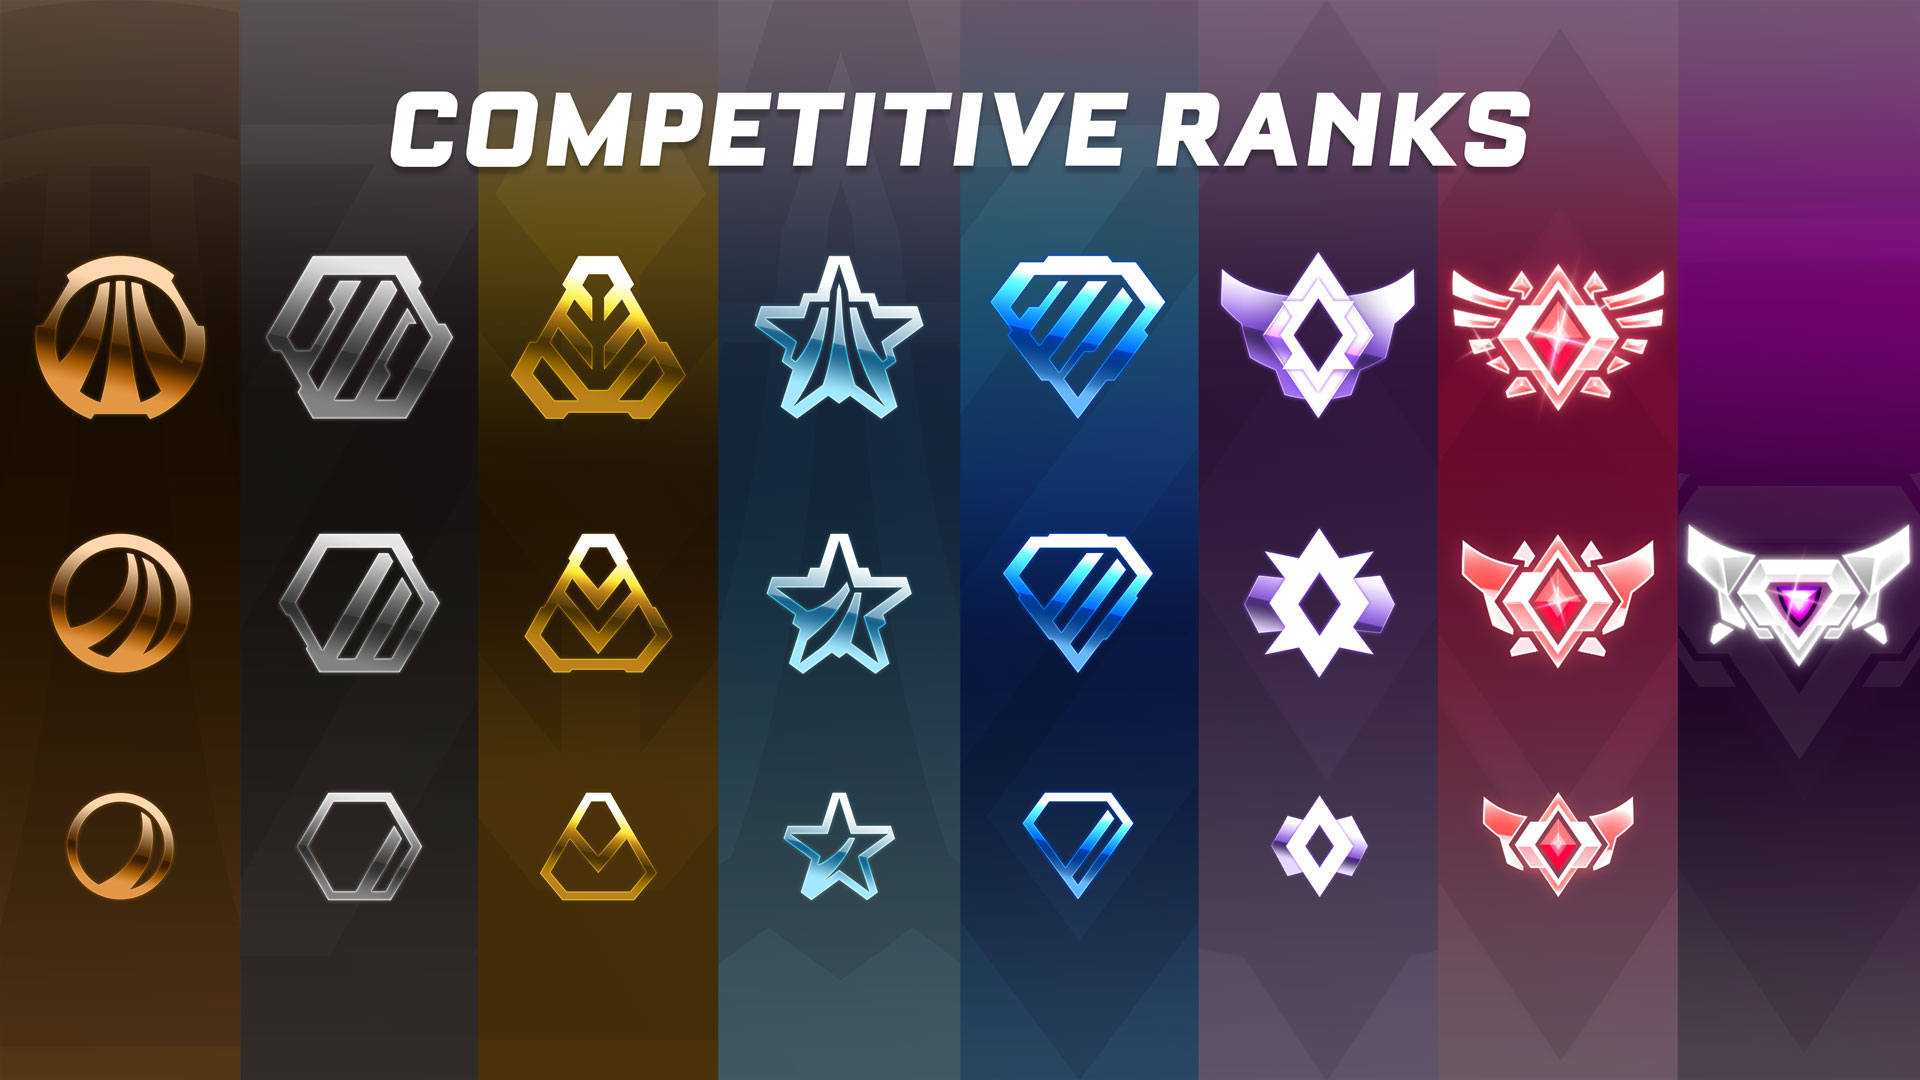
\includegraphics[width=\linewidth]{res/rankings}
    \caption{Rocket league rankings}
    \label{fig:ranks}
\end{figure}

In each modality, the player, after playing 10 competitive- online matches, is classified into a rank, based on the result of the 10 played matches. The ranks (visually shown in \reffig{fig:ranks}) are: 


\begin{multicols}{3}
    \begin{itemize}
        \item Bronze I
        \item Silver I
        \item Gold I
        \item Platinum I      
        \item Diamond I        
        \item Champion I         
        \item Grand Champion I    
        \item Bronze II
        \item Silver II
        \item Gold II       
        \item Platinum II     
        \item Diamond  II         
        \item Champion II         
        \item Grand Champion II
        \item Bronze III
        \item Silver III
        \item Gold III    
        \item Platinum III     
        \item Diamond  III        
        \item Champion III         
        \item Grand Champion III
    \end{itemize}
\end{multicols}

\begin{itemize}
    \item Supersonic Legend
\end{itemize}

Each rank, is split in four divisions (Division I, II, III and IV). And, each rank with its divisions is itself a discretization of a number, that is the Match Making Ranking (MMR). 
The MMR goes from 0 to potentially infinity, however the last rank: Supersonic Legend, takes the interval [1861, +Infinity]. A detailed view on MMRs and rankings is shown in \reftab{tab:mmrs}.

When the player starts playing, it is assigned an MMR of 600, that correspond to Gold III Division II. The MMR increase or decrease basing on the outcome of the matches it plays, obviously if he wins it will increase, viceversa if he loses. How much it can gain or lose at the end of the match is based on the number of played matches. In the first match, the gain/loss is +/-150. In the second match the values is halved, and after, it logarithmically decrease, until after some dozen of matches, it converge to +/- 10.

With this system, the player, will be classified in its most appropriate rank after a few dozen of matches and, therefore will compete with players of the same skill level.
Ranking, is also only determined by the outcome of the match, making the player experience frustrating in some cases. These are the business problems, thus the opportunity is making a more fast ranking system, and also more fair, taking in account the performance of the player in the match, in order to give also a meritocratic system.

\subsection{Determine Business Objectives}

Our business objective is, therefore:
\begin{itemize}
    \item Predict the rank of a player from the skill shown during the match
\end{itemize}
\begin{table}[]
    \begin{tabular}{|l|c|c|c|c|}
    \hline
    \textbf{Tier}                 & \multicolumn{1}{l|}{\textbf{Division I}} & \multicolumn{1}{l|}{\textbf{Division II}} & \multicolumn{1}{l|}{\textbf{Division III}} & \multicolumn{1}{l|}{\textbf{Division IV}} \\ \hline
    \textbf{Supersonic   Legend}  & 1.861 — 2.008                            & —                                         & —                                          & —                                         \\ \hline
    \textbf{Grand Champion   III} & 1.709 — 1.739                            & 1.745 — 1.773                             & 1.788 — 1.814                              & 1.832 — 1.860                             \\ \hline
    \textbf{Grand Champion   II}  & 1.575 — 1.598                            & 1.600 — 1.636                             & 1.638 — 1.660                              & 1.677 — 1.701                             \\ \hline
    \textbf{Grand Champion I}     & 1.435 — 1.458                            & 1.460 — 1.494                             & 1.498 — 1.527                              & 1.537 — 1.559                             \\ \hline
    \textbf{Champion III}         & 1.315 — 1.333                            & 1.335 — 1.366                             & 1.368 — 1.394                              & 1.402 — 1.420                             \\ \hline
    \textbf{Champion II}          & 1.195 — 1.213                            & 1.215 — 1.246                             & 1.248 — 1.275                              & 1.282 — 1.300                             \\ \hline
    \textbf{Champion I}           & 1.075 — 1.093                            & 1.095 — 1.127                             & 1.128 — 1.148                              & 1.162 — 1.180                             \\ \hline
    \textbf{Diamond III}          & 995 — 1.003                              & 1.004 — 1.027                             & 1.028 — 1.051                              & 1.052 — 1.060                             \\ \hline
    \textbf{Diamond II}           & 915 — 923                                & 924 — 947                                 & 948 — 971                                  & 972 — 980                                 \\ \hline
    \textbf{Diamond I}            & 835 — 843                                & 844 — 867                                 & 868 — 891                                  & 892 — 900                                 \\ \hline
    \textbf{Platinum III}         & 773 — 778                                & 779 — 797                                 & 798 — 816                                  & 817 — 825                                 \\ \hline
    \textbf{Platinum II}          & 715 — 718                                & 719 — 737                                 & 738 — 756                                  & 757 — 765                                 \\ \hline
    \textbf{Platinum I}           & 655 — 658                                & 659 — 677                                 & 678 — 696                                  & 697 — 705                                 \\ \hline
    \textbf{Gold III}             & 595 — 598                                & 599 — 617                                 & 618 — 636                                  & 637 — 643                                 \\ \hline
    \textbf{Gold II}              & 535 — 538                                & 539 — 557                                 & 558 — 576                                  & 577 — 585                                 \\ \hline
    \textbf{Gold I}               & 475 — 478                                & 479 — 497                                 & 498 — 516                                  & 517 — 524                                 \\ \hline
    \textbf{Silver III}           & 415 — 418                                & 419 — 437                                 & 438 — 456                                  & 457 — 467                                 \\ \hline
    \textbf{Silver II}            & 355 — 358                                & 359 — 377                                 & 378 — 396                                  & 397 — 414                                 \\ \hline
    \textbf{Silver I}             & 295 — 298                                & 299 — 317                                 & 318 — 336                                  & 337 — 354                                 \\ \hline
    \textbf{Bronze III}           & 235 — 238                                & 239 — 257                                 & 258 — 276                                  & 277 — 290                                 \\ \hline
    \textbf{Bronze II}            & 172 — 178                                & 179 — 197                                 & 198 — 216                                  & 217 — 233                                 \\ \hline
    \textbf{Bronze I}             & 0 — 118                                  & 121 — 137                                 & 140 — 155                                  & 157 — 172                                 \\ \hline
    \end{tabular}
    \caption{MMRs intervals related to each Division and Rank in Rocket League}
    \label{tab:mmrs}
\end{table}

This work will result in a system able to measure the skill shown in a match for each player in a "short" amount of time, in order to be implemented in a real system.
The business success criteria are:
\begin{itemize}
    \item Positive feedback by the community after its implementation;
    \item Increase in daily active players by 5\%.
\end{itemize}

However, a business expert should be required to better quantify the success criteria.

\subsection{Determine Data Mining Goals}
\label{sec:min_goal}
The goal is a classification/regression task, therefore a prediction task. There are 22 ranks, or we can possibly group by in 8, (bronze, silver, gold, platinum, diamond, champion, grand champion, SSL), therefore, it could be a classification task. On the other hand we would lose the natural ordering of the classes, furthermore, the ranks are a discretization of the MMR, that is a numeric continuous variable. Thus, the more appropriate task is regression.

The criteria will be based on RMSE and MAE, it will be accepted a MAE inferior to 2.0 and a RMSE inferior to 2.5. 
Another criteria is the inference time on 6 examples (number of players in a match), that should be less than 0.5 seconds, measured on a CPU AMD Ryzen 2600x.
